\section{Software-Sensor-Based Attack Detection and Recovery Methodology}

Figure~\ref{fig:phase7_pipeline} summarizes the proposed software-sensor-based attack detection and recovery pipeline. The V9 trained hybrid software sensor predicts the future state $\hat{x}_{V9}[k+1]$ using information available at time $k$. The predicted future state is compared with the measured future state $x_{measured}[k+1]$ to compute the residual. For Roll and Pitch, the residual is computed using direct subtraction. For Yaw, circular angular difference is used to handle angular wrap-around.

\begin{figure*}[t]
    \centering
    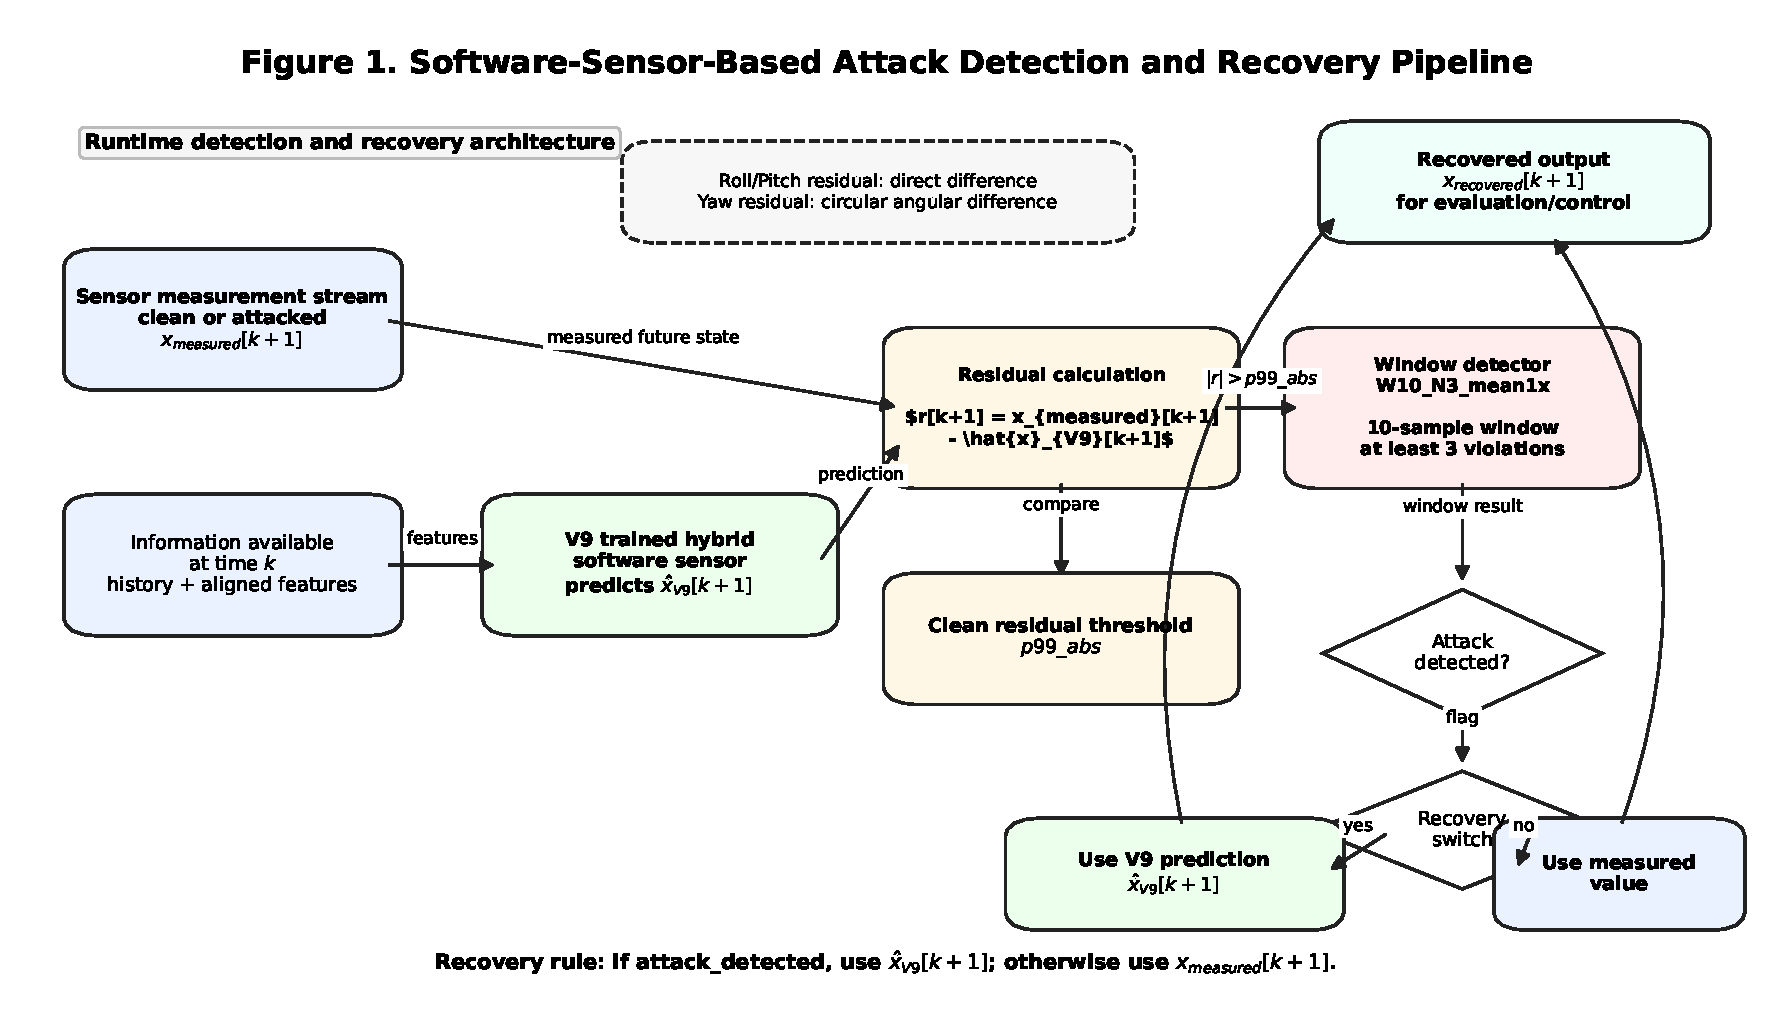
\includegraphics[width=0.95\textwidth]{phase7_methodology_figures/figure1_detection_recovery_pipeline.pdf}
    \caption{Software-sensor-based attack detection and recovery pipeline. The V9 trained hybrid predictor estimates the future state, the residual is compared against the $p99\_abs$ threshold, and the W10\_N3\_mean1x detector determines whether the recovery switch should replace the attacked measurement with the software-sensor prediction.}
    \label{fig:phase7_pipeline}
\end{figure*}

Figure~\ref{fig:phase7_workflow} shows the complete training and deployment workflow. Clean baseline logs are used to train and evaluate candidate predictors, select the V9 trained hybrid predictor, generate clean residuals, and compute the $p99\_abs$ threshold. The selected predictor and threshold are then deployed on attacked logs for detection, recovery, and RMSE/MAE evaluation.

\begin{figure*}[t]
    \centering
    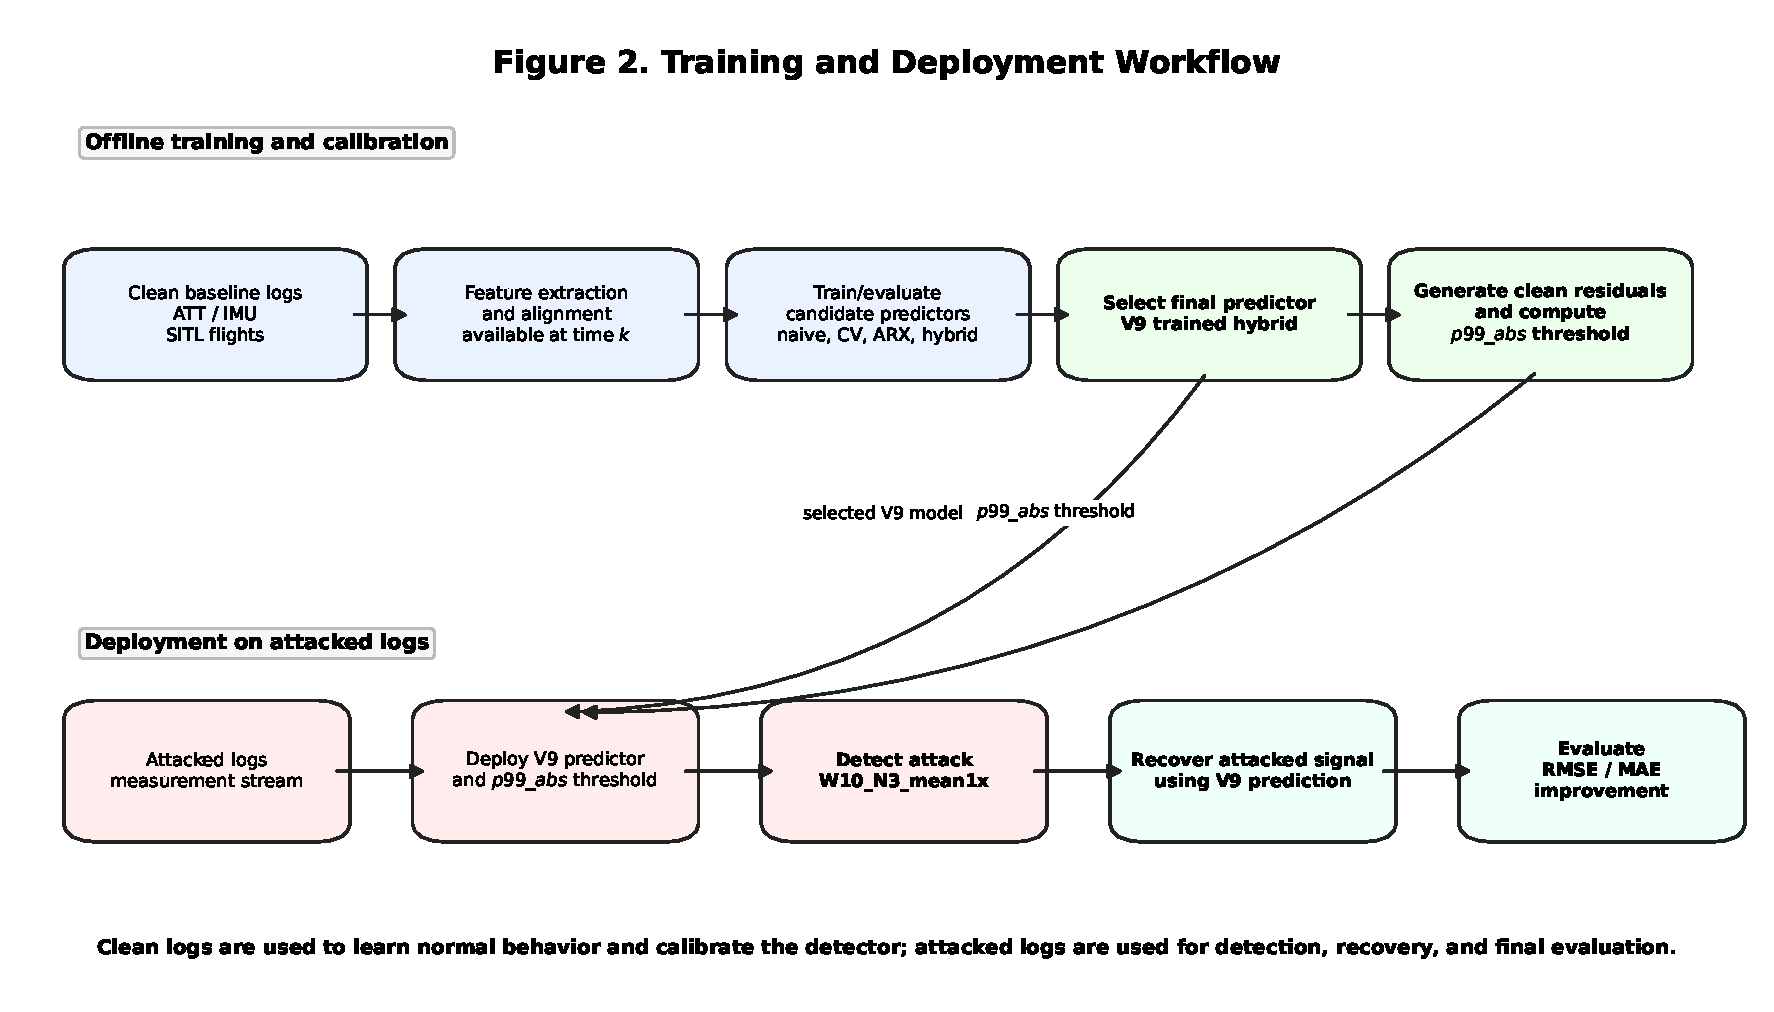
\includegraphics[width=0.95\textwidth]{phase7_methodology_figures/figure2_training_deployment_workflow.pdf}
    \caption{Training and deployment workflow for the software-sensor recovery system. Clean logs are used for predictor selection and threshold calibration, while attacked logs are used for detection, recovery, and quantitative evaluation.}
    \label{fig:phase7_workflow}
\end{figure*}

Figure~\ref{fig:phase7_v9_internal} illustrates the internal structure of the V9 trained hybrid software sensor. V9 combines a naive predictor, a constant-velocity predictor, and an ARX-style predictor using validation-based weights:

\[
\hat{x}_{V9}[k+1] =
w_{naive}\hat{x}_{naive}[k+1]
+ w_{cv}\hat{x}_{cv}[k+1]
+ w_{arx}\hat{x}_{arx}[k+1].
\]

\begin{figure*}[t]
    \centering
    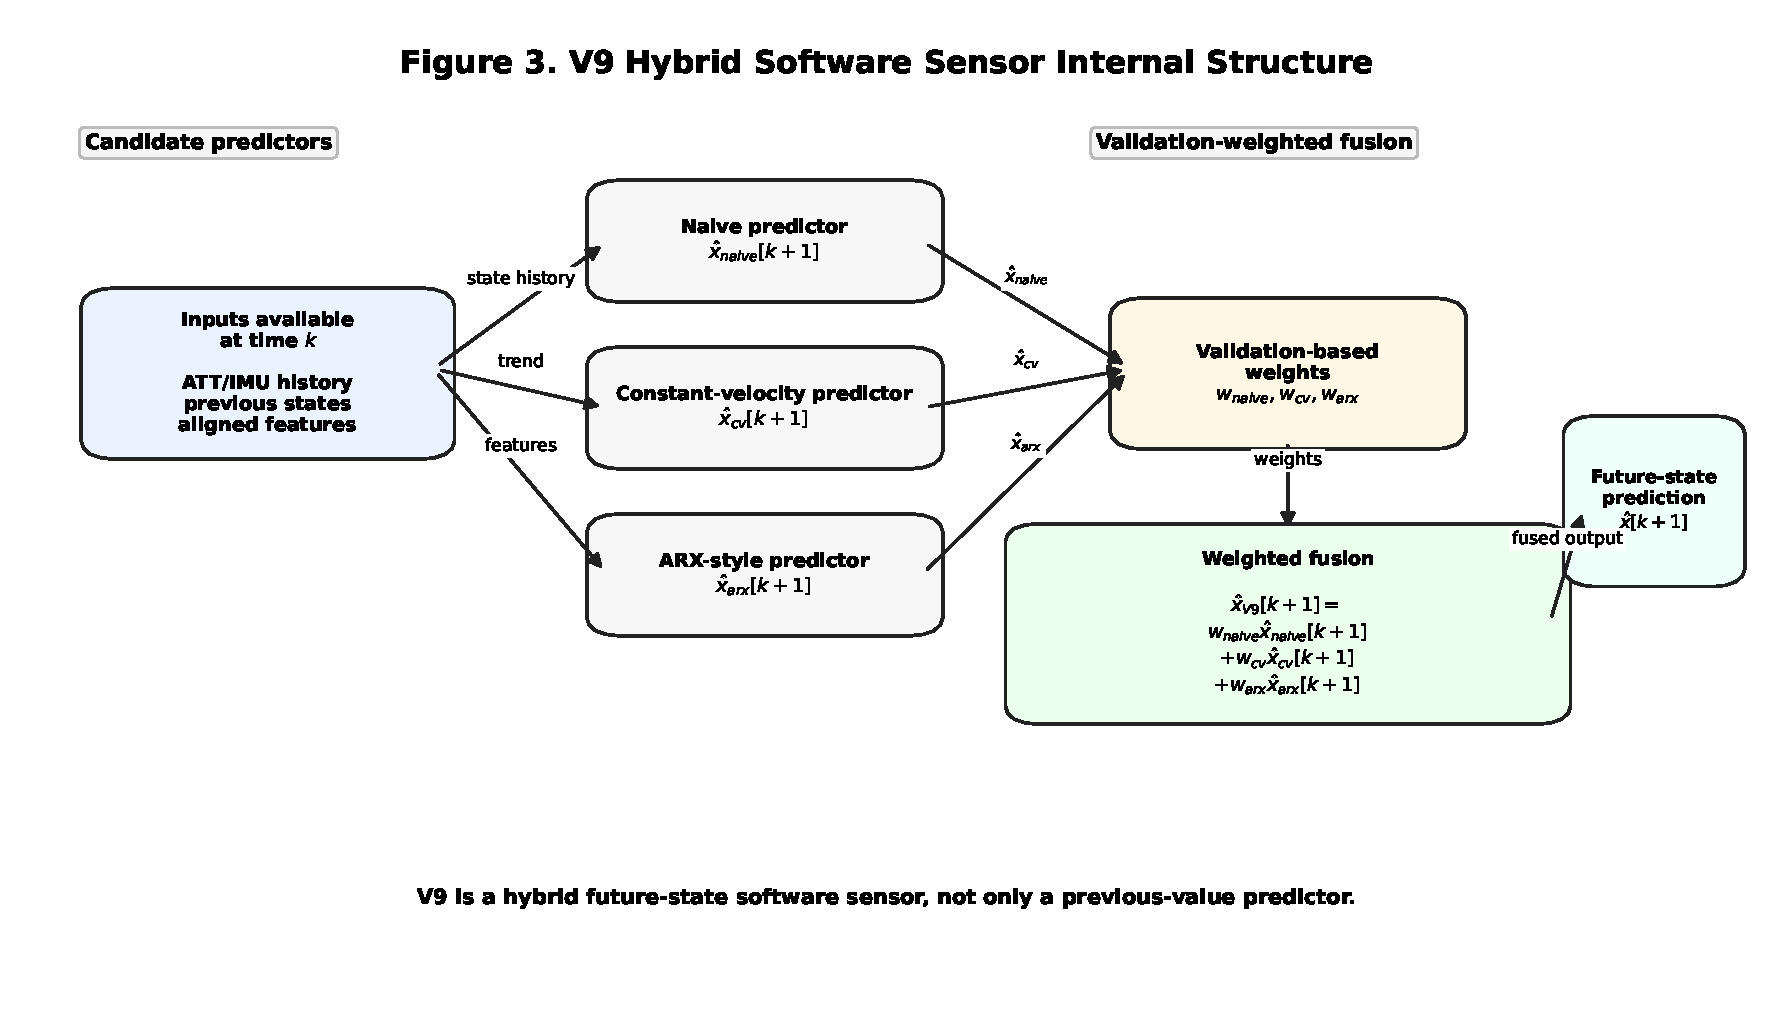
\includegraphics[width=0.95\textwidth]{phase7_methodology_figures/figure3_v9_hybrid_internal_structure.pdf}
    \caption{Internal structure of the V9 trained hybrid software sensor. The final future-state estimate is produced by validation-weighted fusion of naive, constant-velocity, and ARX-style predictions.}
    \label{fig:phase7_v9_internal}
\end{figure*}

Figure~\ref{fig:phase7_window_detector} presents the residual and window-based detection logic. The absolute residual is compared with the $p99\_abs$ threshold. The W10\_N3\_mean1x detector declares an attack when at least three threshold violations occur within a ten-sample window.

\begin{figure*}[t]
    \centering
    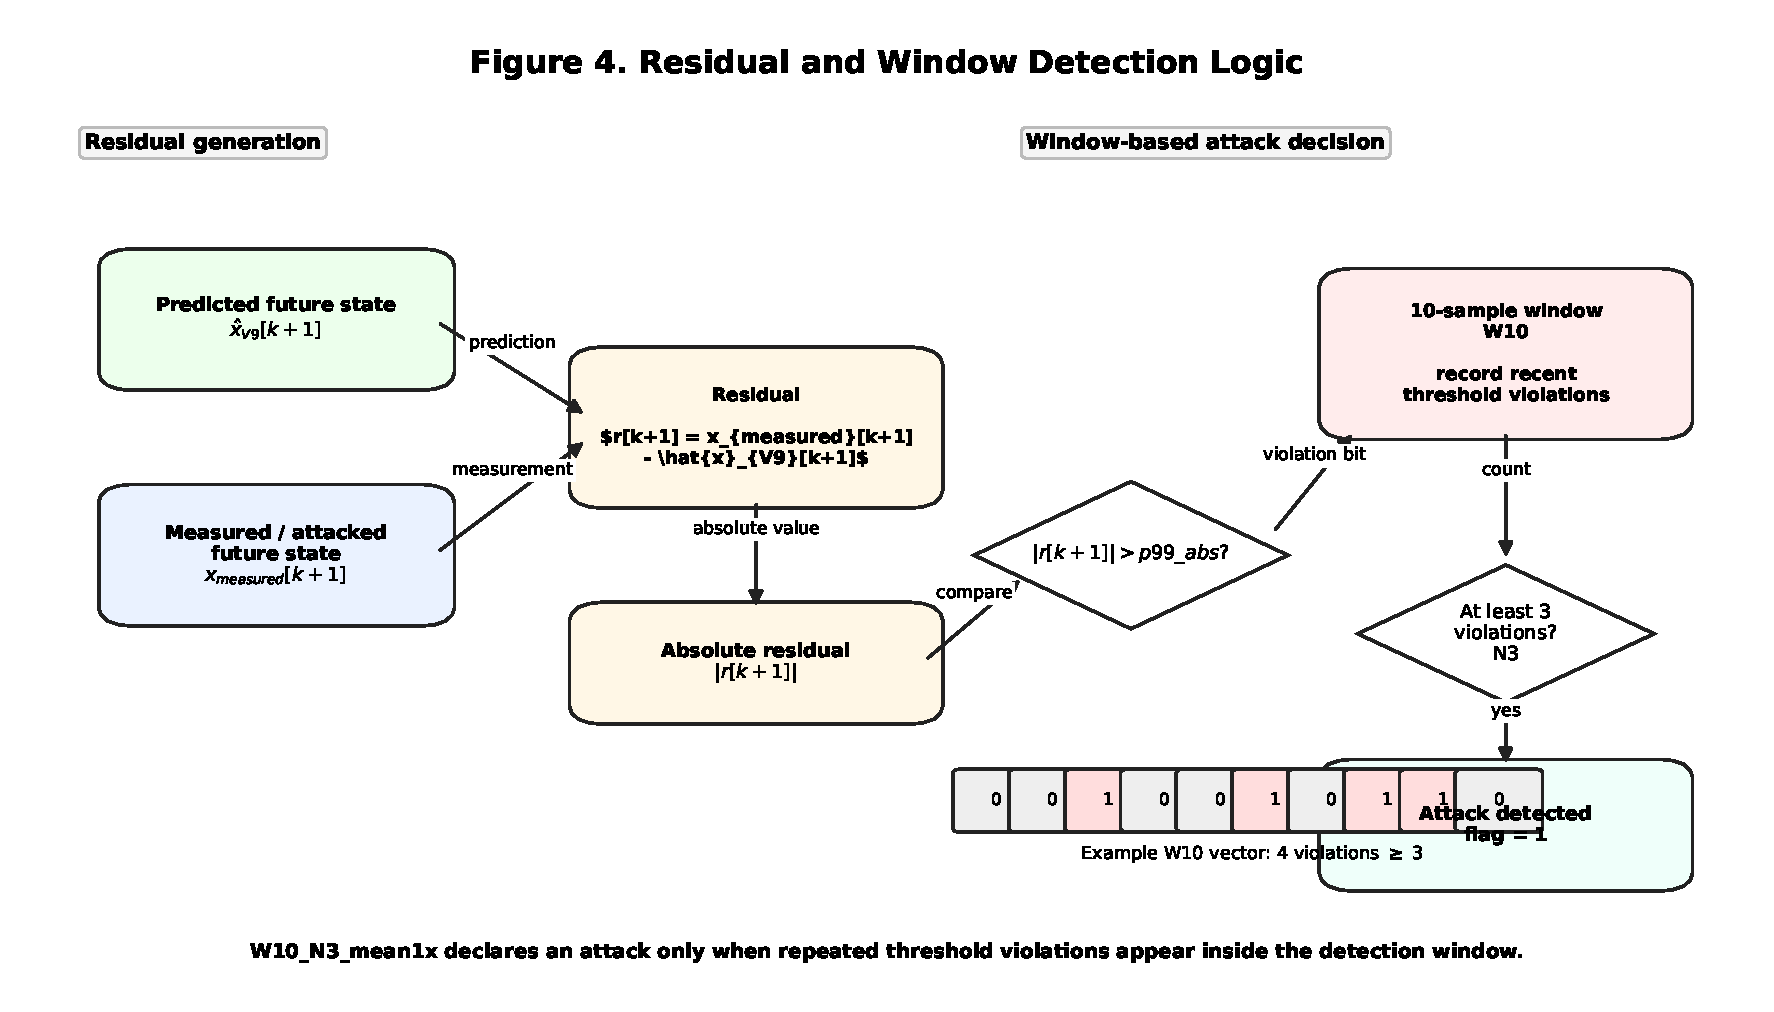
\includegraphics[width=0.95\textwidth]{phase7_methodology_figures/figure4_residual_window_detection_logic.pdf}
    \caption{Residual and window-based detection logic. The detector uses the $p99\_abs$ threshold and declares an attack when repeated threshold violations occur inside a ten-sample window.}
    \label{fig:phase7_window_detector}
\end{figure*}

Figure~\ref{fig:phase7_recovery_switch} shows the recovery decision logic. When an attack is detected, the recovered signal is replaced by the V9 prediction. Otherwise, the original measured signal is preserved:

\[
x_{recovered}[k+1] =
\begin{cases}
\hat{x}_{V9}[k+1], & \text{if attack\_detected},\\
x_{attacked}[k+1], & \text{otherwise}.
\end{cases}
\]

\begin{figure*}[t]
    \centering
    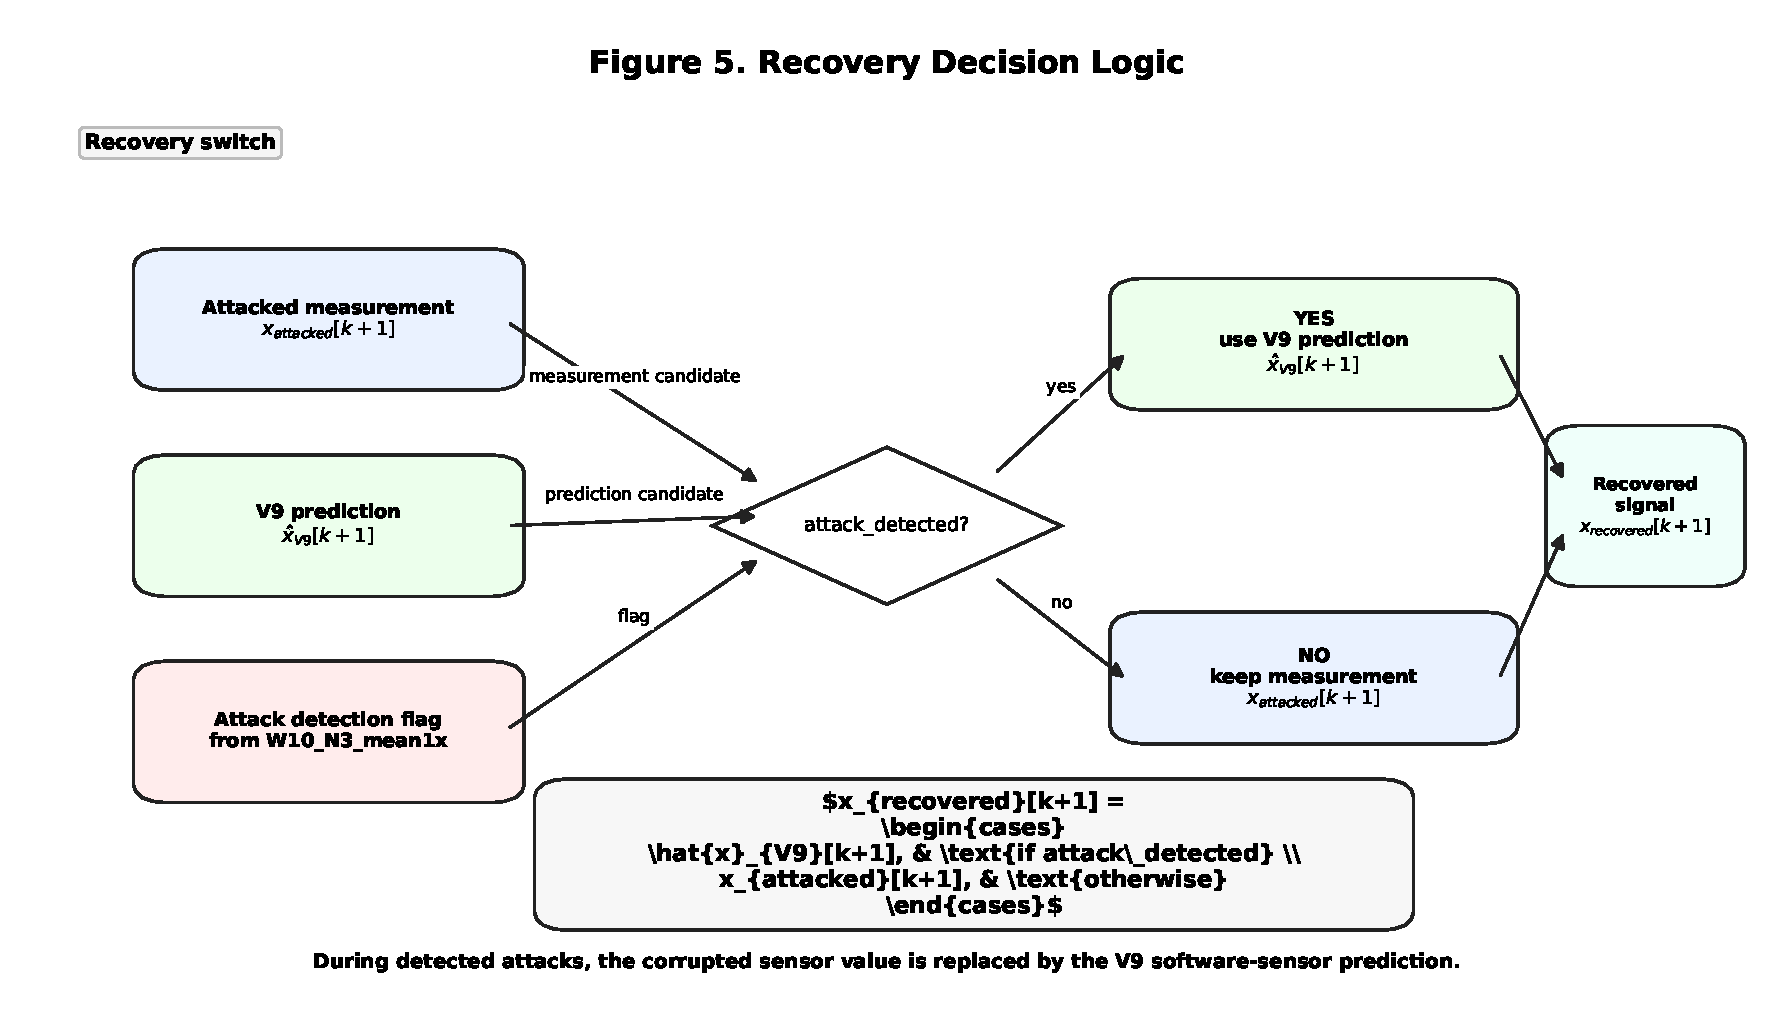
\includegraphics[width=0.95\textwidth]{phase7_methodology_figures/figure5_recovery_decision_logic.pdf}
    \caption{Recovery decision logic. The recovery switch substitutes the attacked measurement with the V9 software-sensor prediction only when the detector flags an attack.}
    \label{fig:phase7_recovery_switch}
\end{figure*}
